\documentclass{article}
\title{Project \#1}
\author{Illya Starikov}
\date{Due Date: March 25, 2016}

\usepackage[english]{babel}
\usepackage{graphicx}
\usepackage[utf8]{inputenc}
\usepackage{menukeys}

\usepackage{hyperref}
\hypersetup{
    colorlinks=true,
}


\usepackage{xcolor}
\newcommand{\shellcmd}[1]{\texttt{\colorbox{gray!30}{#1}}}

\begin{document}
\maketitle

\setcounter{section}{-1}

\section{Introduction}
\begin{itemize}
    \item Install 2 editor plugins
    \item Document 5 editor features (with vim, this'll be a cinch)
    \item Do the job control section of project B (I use this all the time)
    \item What does the -exec option on find do?
    \item What does xargs do?
    \item Look up and use tmux.
\end{itemize}

\section{Two Editor Plugins}
For two text editors plugins, I chose (facetiously) pathogen and powerline.

\subsection{pathogen.vim}
Naturally when I knew I was going to install packages, my first thought was to use a package manager. Easily manipulating and deleting new packages was going to be critical, so Pathogen looked to be the proper choice.

\subsubsection{What It Does}
In its simplest terms, pathogen makes package management as easy as \shellcmd{rm -r}. My main use has been mostly to easily locate and delete new plugins that I do not use in my \texttt{bundle} directory.

\subsubsection{How To Use It}
After \href{https://github.com/tpope/vim-pathogen#runtime-path-manipulation}{initial setup}, pathogen actually does the rest.

\subsection{Powerline}
While on my quest to find text editor plugins, I stumbled upon and installed powerline. While trying to think of my second plugin to write in this report, I couldn't help but notice how much I was using Powerline.

\subsubsection{What It Does}
Powerline is an alternative to the standard Vim statusline.

\begin{figure}[!ht]
    \centering
    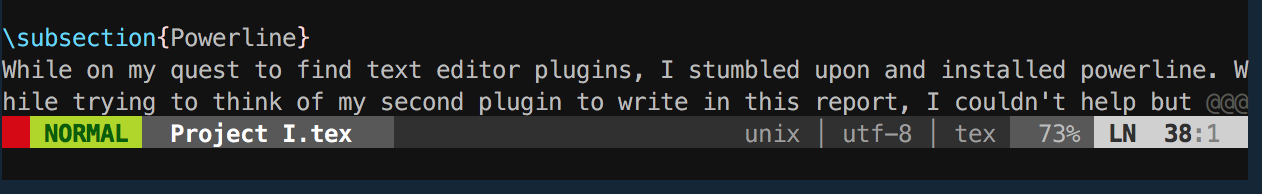
\includegraphics[width=0.85\textwidth]{assets/powerline.png}
    \caption{The Powerline In Action}
\end{figure}

It changes the configuration based on the mode that you are.

\subsubsection{How To Use It}
Use of powerline is automatic.

\section{Five Editor Features}
For my five editor features, I decided to do:


\begin{description}
    \item [External commands (\keys{r}\keys{!}\shellcmd{Command})] To run an external command outside of vim, and pipe the input back into the file. Makes inserting the date into \LaTeX documents much, much faster.
    \item [Searching (\keys{\slash} \keys{?})] \keys{Command}\keys{F} for Vim.
    \item [Go to line (\texttt{:number})] Jumping to a specified line number.
    \item [Autocomplete (\keys{control}+\keys{n})] Attempts to finish the work being typed (whether it be a command or variable)
    \item [Text folding (\keys{z}+\keys{f})a]
\end{description}

\section{Job Control}
\begin{enumerate}
    \item It terminates.
    \item It terminates the command from the background.
    \item Waits until all previous processes have finished until continueing.
\end{enumerate}

\section{Find \shellcmd{exec}ution}
According to \shellcmd{Man},

\begin{verbatim}
-exec utility [argument ...] ;
      True if the program named utility returns a zero value as its exit
      status.  Optional arguments may be passed to the utility.  The
      expression must be terminated by a semicolon (``;'').  If you
      invoke find from a shell you may need to quote the semicolon if the
      shell would otherwise treat it as a control operator.  If the
      string ``{}'' appears anywhere in the utility name or the arguments
      it is replaced by the pathname of the current file.  Utility will
      be executed from the directory from which find was executed.
      Utility and arguments are not subject to the further expansion of
      shell patterns and constructs.
\end{verbatim}

Essentially \shellcmd{exec} allows the \shellcmd{exec}ution of certain programs during a command. For example, to make the use relevant to \shellcmd{find}, searching for an instance of a keyword in open files would \shellcmd{find . -exec grep KEYWORD {} +}.


\section{\textit{T}erminal \textit{Mu}ltiple\textit{x}or}
Finished, used for the job controls section (SSH to tmux to logout).

\section{Xargs}
Back to \shellcmd{Man},

\begin{verbatim}
The xargs utility reads space, tab, newline and end-of-file delimited
strings from the standard input and executes utility with the strings as
arguments.

Any arguments specified on the command line are given to utility upon each
invocation, followed by some number of the arguments read from the standard
input of xargs.  The utility is repeatedly executed until standard input is
exhausted.

Spaces, tabs and newlines may be embedded in arguments using single
(`` ' '') or double (``"'') quotes or backslashes (``\'').  Single quotes
escape all non-single quote characters, excluding newlines, up to the
matching single quote.  Double quotes escape all non-double quote charac-
ters, excluding newlines, up to the matching double quote.  Any single
character, including newlines, may be escaped by a backslash.
\end{verbatim}

\shellcmd{xargs} allow for the manipulation of standard input, becoming quite useful with commands such as \shellcmd{find} or \shellcmd{ls}.

\section{Conclusion}
In conclusion, I have gained more familiarity with the command line. To take the assignment another step up, the entirety of this assignment has been created using the command line — Vim, \texttt{pdflatex}, \texttt{rm} for removing of \LaTeX files, etc.
\end{document}
